% \Image{Capa do livro (; )}{PNLD2022-001-01.png}
% \Image{Ilustração do livro (Acorde/Manuella Silveira; Acorde)}{PNLD2022-001-04.png}
% \Image{Ilustração do livro (Acorde/Manuella Silveira; Acorde)}{PNLD2022-001-05.png}
% \Image{Ilustração do livro (Acorde/Manuella Silveira; Acorde)}{PNLD2022-001-06.png}

\documentclass[11pt]{extarticle}
\usepackage{manualdoprofessor}
\usepackage{fichatecnica}
\usepackage{lipsum,media9}
\usepackage[justification=raggedright]{caption}
\usepackage[one]{bncc}
\usepackage[ayllon]{../edlab}
\usepackage{marginnote}
\usepackage{pdfpages}

\newcommand{\AutorLivro}{Klévisson Viana}
\newcommand{\TituloLivro}{Viagem ao reino encantado do cordel}
\newcommand{\Tema}{Diversão e aventura}
\newcommand{\Genero}{Cordel}
%\newcommand{\imagemCapa}{./images/PNLD2022-001-01.jpeg}
\newcommand{\issnppub}{XXX-XX-XXXXX-XX-X}
\newcommand{\issnepub}{XXX-XX-XXXXX-XX-X}
% \newcommand{\fichacatalografica}{PNLD0001-00.png}
\newcommand{\colaborador}{Paulo Pompermaier}

\begin{document}

\title{\TituloLivro}
\author{\AutorLivro}
\def\authornotes{\colaborador}

\date{}
\maketitle

\tableofcontents

\begin{abstract}
Este material tem a intenção de contribuir para que você consiga desenvolver um trabalho aprofundado com a obra \textit{Viagem ao reino encantado do cordel} em sala de aula.
Você encontrará informações sobre o autor, sobre o gênero e também 
algumas propostas de trabalho para a sala de aula que você poderá explorar livremente, 
da forma que considerar mais apropriada para os seus estudantes.

O autor desse cordel, Klévisson Viana, é um dos principais cordelistas contemporâneos.
Nascido em Quixeramobim, interior do Ceará, desde pequeno o autor entrou em contato com o universo do cordel.
Além de escrever e publicar diversos poemas de cordel, Klévisson é um nome importante do universo cordelista pelo importante papel de divulgação que exerce: ilustra, diagrama e edita diversas obras de cordelistas do nordeste. 
Após fundar a editora Tupynanquim, em 1995, já publicou e divulgou centenas de cordéis pelo Brasil.

Podemos perceber sua inserção e seu amor pelo universo do cordel neste
\textit{Viagem ao reino encantado do cordel}. Resgatando o clássico \textit{Romance do pavão misterioso}, o poema funciona como uma grande homenagem aos diversos cordéis que marcaram a vida e o imaginário de milhares de leitores sertão adentro. Desde o início, clássicos do gênero são citados e, logo depois, as protagonistas da história partem em uma aventura através da qual visitam e assistem a diversos eventos narrados nas obras de cordel invocadas. Ao final da viagem, o pavão que transporta os aventureiros ainda fala brevemente sobre a origem do cordel, sua função e inserção no ambiente cultural e social do Nordeste.
Além das aventuras cativantes, a obra apresenta-se portanto como uma boa porta de entrada para o reino encantado do cordel: apresenta suas narrativas mais representativas, segue as características típicas da linguagem de cordel, fala sobre sua história, e tudo ilustrado com as clássicas gravuras em madeira, ou xilogravuras.

Ao longo do manual, todos esses aspectos serão explorados e relacionados a sugestões de atividades. Com isso, objetiva-se oferecer algumas ideias e inspirações para um trabalho que pode ser desenvolvido tanto a curto, quanto a médio e longo prazo. Sinta-se à vontade para personalizar a aula e torná-la sua, aplicando seus conhecimentos, sua 
personalidade e aproveite para fortalecer seu vínculo com a turma.

Boa aula!
\end{abstract}

\SideImage{Típica capa de um cordel feita a partir da gravura em madeira, a xilogravura (CC-BY-SA-4.0)}{PNLD2023-004-06.jpg}

\section{Sobre o livro}
O livro \textit{Viagem ao reino encantado do cordel}, como o próprio nome indica, é um cordel de Klévisson Viana, ilustrado com xilogravuras de Maércio Siqueira. Pelo diálogo constante que estabelece com narrativas clássicas do cordel, pode-se ver essa história como uma grande homenagem ao universo do cordel e às histórias consagradas pelos grandes cordelistas. A narrativa começa em uma Fazenda de Ouro Preto, onde a avó Alzira mostra para seus netos, Miguel, Maria e Kahlil, uma maleta cheia de cordéis.

Diversos clássicos do gênero são citados, como a história de João Grilo, Canção de Fogo, Malasartes, a Donzela Teodora, Pedro Cem, Juvenal e o Dragão etc. Mas a principal história, contada e recontada diversas vezes pela avó, é do pavão misterioso: no cordel de José Camelo de Melo Rezende, narra-se a aventura de Evangelista que, enamorado de uma princesa grega, encomenda uma maquinaria engenhosa que o permita chegar ao quarto onde a princesa Creusa fica encarcerada e escondida pelo pai ciumento. Com seu pequeno aeroplano, em formato de pavão, Evangelista consegue chegar à Creusa, tirá-la da torre e casar-se com ela. O rei, afinal, falece, e Evangelista herda sua fortuna, vivendo feliz para sempre ao lado da esposa Creusa e do irmão que o apoiou em sua aventura.

Mas tal narrativa é apenas insinuada no cordel de Klévisson Viana, não sendo abordada inteira. Após a cena da avó com os netos, passa-se à descrição do vovô Manoel Lima: comerciante da região, seu armazém é descrito em minúcia, com todos os secos e molhados que dispunha para os moradores da vila. Entra em cena, então, seu Salim, velho turco que vem fazer negócios com Manoel. O mascate traz mercadorias de longe e, numa negociação um pouco suspeita, vende um lote de produtos para Manoel, que os guarda no galpão de seu armazém.

Ali, por curiosidade, as crianças avistam uma estranha maleta. Ao apertar um botão da caixa, monta-se um aeroplano em forma de pássaro. Eles então sobem no pavão e começam a voar. O pavão fala enquanto sobrevoa. Conta como tudo começou na Turquia e na Grécia, quando for construído a pedido de Evangelista, e como ele depois se casou com Creusa. Após cumprir sua função, ficara esquecido em um canto, até venderem-no para Salim e, assim, chegar até as crianças. Durante o voo, o pavão faz várias paradas nos diversos reinos nos quais se passam as histórias de cordel citadas ao início do livro. Assim, as crianças presenciam a luta de Juvenal e seus três cães contra o dragão; a incrível memória da escrava Teodora, de Túnis; as aventuras sertanejas de João Grilo e Lampião.

Depois da viagem com tantas aventuras, os meninos querem saber mais sobre os cordéis. Então o pavão lhes conta como nasce esse tipo de literatura, sua relação com o trovadorismo, como circulava, para que servia. Ao final, as crianças voltam para o galpão, o pavão fecha-se novamente em sua maleta, e guardam para sempre as histórias que ouviram e viveram naquele dia.


\reversemarginpar
\marginparwidth=5cm

%\marginnote{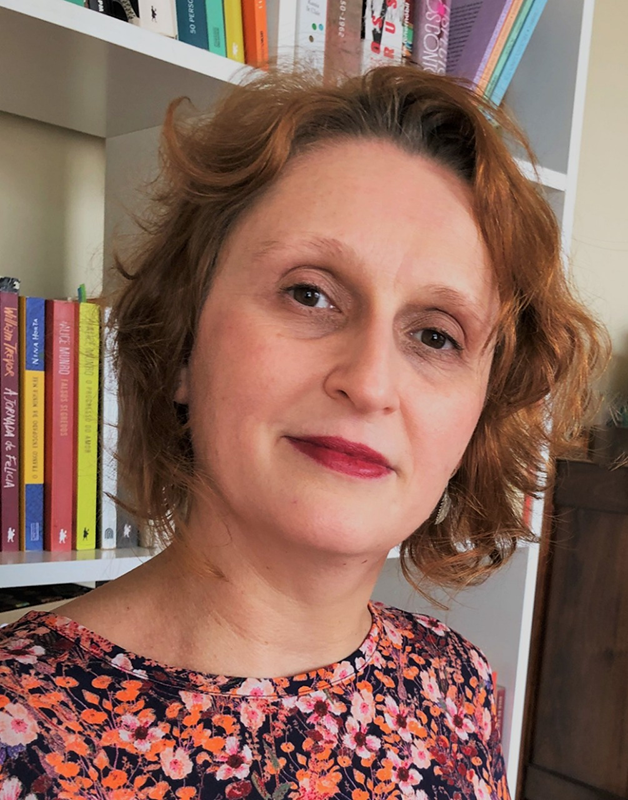
\includegraphics[width=\marginparwidth]{./images/PNLD2022-001-02.png}\\
%A autora Camila Werner (Arquivo pessoal)}


\section{Sobre o autor}


%532 caracteres
Klévisson Viana nasceu em 3 de novembro de 1972 no interior do Ceará, na cidade de Quixeramobim. Além de escrever poesia em cordel, ele desenha, diagrama, imprime e comercializa suas obras, tendo um papel ativo na publicação e divulgação da obra de diversos cordelistas. Em 1980, aos oito anos, Klévisson mudou-se com a família para Canindé, tendo estudado apenas até o primeiro ano do segundo grau.

Canindé, a essa época, era uma espécie de centros da devoção popular da fé católica, congregando crentes, artistas sacros e vendedores de imagens católicas não
apenas do Ceará, mas do Nordeste inteiro. De família camponesa humilde, Klévisson ingressou nesse grande mercado de Canindé aos nove anos, vendendo bombons, artigos religiosos e velas nas datas e ocasiões especiais, como no Dia dos Finados.
Ali se tornou amigo dos diversos cordelistas que vinham a Canindé vender suas obras para os romeiros.

Apesar disso, sua relação com a arte e a literatura de cordel já vinha de sua família, como nos relembra José Nêumanne:

\begin{quote}
Sua avó paterna era uma pessoa esclarecida, dada a leituras, e havia inoculado no pai dele um gosto especial pelos romances de aventura, humor, conhecimento e fé, contidos nos folhetos comprados em feiras. A família era possuidora de um acervo razoável desses folhetos, que o pai costumava ler para os filhos quando voltava do trabalho duro --- de sol a sol, como se diz por lá --- de semear e colher no semiárido.\footnote{``Introdução''. Em: \textit{Biblioteca de Cordel: Klévisson Viana}. São Paulo: Hedra, 2007, p. 11.}
\end{quote}

Aos 14 anos, Klévisson ingressou de vez no universo da arte, fazendo ilustrações para os jornais de bairro de Canindé. Nessa mesma época, promovia salões de humor e eventos culturais na cidade. Na década de 1990, mudou-se para a capital, Fortaleza, onde passou a integrar diversos eventos e manifestações de artistas e humoristas cearenses.

Continuou, ainda assim, a colaborar na imprensa. Entre 1990 e 1995, foi ilustrador do jornal \textit{O povo}. Junto ao jornalista Tarcísio matos, foi editor da página \textit{Muro baixo}, na qual publicava charges, cartuns, caricaturas e piadas. Outro jornal de Fortaleza, a
\textit{Tribuna do Ceará}, também recebeu diversas colaborações textuais e desenhos seus.

Do formato clássico do cordel, logo passou a experimentar outras formas artísticas. Através da influência do irmão, Arievaldo Viana, descobriu seu talento como quadrinista, que o levaria a ganhar o prêmio nacional \textsc{hq} Mix, o mais importante do país no que se refere às histórias em quadrinhos, em 1998. Na ocasião, foi premiado por sua obra \textit{Lampião\ldots{} Era o cavalo do tempo atrás da besta da vida}, que reconta a vida e aventura do famoso cangaceiro em formato de quadrinho.

A primeira edição da obra foi publicada por uma então desconhecida gráfica e editora cearense, a Tupynanquim Aldeia, Mídia \& Tal, fundada por Klévisson e alguns amigos. Através da Tupynanquim, o artista passou a editar e publicar seus próprios folhetos de cordel, além de publicar e divulgar a obra de outros cordelistas. Desde sua fundação, em 1995, sua editora publicou mais de cinquenta poetas do Brasil inteiro.


\paragraph{A obra de Klévisson Viana}
Multiartista, agitador cultural, editor, Klévisson Viana também imprimiu essa heterogeneidade à sua produção poética. Em suas pesquisas na memória sertaneja do cangaço, o artista se aprofundou  nas tradições da poesia popular unindo-as a experimentações em diferentes gêneros artísticos. 
Tendo em vista a diversidade de sua produção, o pesquisador José Nêumanne propõe uma divisão de sua obra em alguns eixos temáticos:

\noindent\textsc{o repórter}: Na tradição do cordel, muito verso é criado de improviso em cima de acontecimentos da realidade. Nos rincões do país, com a difícil circulação de jornais, a falta de acesso ao rádio e à televisão, os sertanejos tinham o costume de se informar sobre os fatos cotidianos através dos cordéis e romances adquiridos nas feiras semanais de sua cidade.
No caso de Klévisson, sua produção cordelística não ignorou essa típica matriz de produção poética. Assim, entre seus diversos títulos, pode-se relembrar um cordel sobre a guerra entre os Estados Unidos e o Iraque; sobre a notícia de jumentos vendidos a R\$ 1,00; sobre 
os atentados terroristas que demoliram as Torres Gêmeas em Nova York e parte do Pentágono, em Washington, em 11 de setembro de 2001; sobre a morte de Celso Daniel, prefeito de Santo André e coordenador do programa de governo da campanha de Lula (\textsc{pt}) à Presidência da República; além da própria vitória eleitoral de Lula em novembro de 2002, também tematizado em sua obra.

\noindent\textsc{o romancista}: Da mesma forma que não chegavam jornais ao interior nordestino, também eram escassos os livros, com exceção das igrejas e casas paroquiais.
Nesse cenário, abundavam os cordéis fantásticos, que abordavam narrativas clássicas, temas mitológicos e medievais, típicos dos romances. 
Klévisson, como anota José Nêumanne, não ficou de fora dessa produção também:

\begin{quote}
O jovem cearense mostra-se um fabulador à altura de clássicos como \textit{O pavão mysteriozo} ou \textit{O país de São Saruê}, no recriar as viagens de aventuras de Hércules e outros heróis mitológicos, a partir de padrões fixados na literatura medieval europeia e reproduzida nos folhetos de cordel de antigamente. Merecem ser destacados dois títulos: \textit{O boi dos chifres de ouro ou O vaqueiro das três virtudes} e \textit{O príncipe do Oriente e o pássaro misterioso}.\footnote{\textit{Ibidem}, p. 21.}
\end{quote}

\noindent\textsc{o quengo}: Na definição sertaneja, ``quengo'' refere-se aos nordestinos que conseguem fugir da desgraça com ginja, malemolência e graça. Talvez sua figura mais conhecida seja João Grilo, eternizado pela peça de Ariano Suassuna, \textit{O auto da Compadecida}, e o posterior filme homônimo. Em Klévisson, podem-se encontrar a clássica figura do quengo em cordéis como \textit{Viagem ao país de São Cornélio} e \textit{O rapaz que namorou com a velha dos papangus pensando que era a Carla Perez}. 


\noindent\textsc{o historiador}: Klévisson também abordou muito a história e a biografia em suas obras. Além do \textsc{hq} já mencionado sobre Lampião, com a típica temática do cangaço, o autor também versou sobre personalidades de outras artes, como o cinema, no caso do cordel \textit{Charlie Chaplin, o Carlitos: do Big Bem à Coluna da Hora}.

\noindent\textsc{o inventor de episódios}: Outra característica da literatura de cordel é a reprodução de desafios de repentistas. Talvez o cordel que siga essa temática que mais obteve sucesso foi o folheto versando sobre a peleja entre o Cego Aderaldo e Zé Pretinho. Klévisson também frequenta o gênero, com cordéis como \textit{A insustentável
peleja de Zé Maria de Fortaleza com Calixtão de Guerra}, \textit{A grande peleja virtual de Klévisson Viana com Rouxinol do Rinaré} e \textit{A grande peleja de Beneval com José Mota Pinheiro}.

\noindent\textsc{o adaptador}: Por fim vale lembrar o frequente hábito entre os cordelistas de adaptar históricas clássicas de romances, de lendas medievais europeias ou da Grécia Antiga, e inclusive dos próprios colegas cordelistas. Entre sua vasta obra, podemos citar a adaptação que Klévisson fez de Homero, em \textit{Helena de Troia e o cavalo misterioso}, de histórias da carochinha com \textit{A história de João e o pé de feijão} e do cordelista Zé Pacheco, escrevendo uma espécie de continuidade para seu clássico \textit{A festa dos cachorros} com \textit{O divórcio da cachorra}.

\paragraph{A autora}
Arlene Holanda nasceu em Limoeiro do Norte, no Ceará. Conviveu durante sua infância com o universo mágico do cordel. Entre suas história preferidas, estão a do Pavão e de
Juvenal. A curiosidade e o gosto por histórias me fizeram-na escolher o curso de História. Especializou-se também em Artes Visuais. Escreve em variados gêneros e estilos literários. Tem cerca de 50 livros publicados, entre literatura (adulto, infantil e juvenil), didáticos e obras complementares.

\paragraph{O ilustrador}
Maércio Siqueira nasceu em Santana do Cariri, Ceará, em 21 de novembro de 1977.
Mora em Crato, Ceará, desde os cinco anos. No Curso de Letras, em 1999, conheceu o
maravilhoso mundo da literatura de cordel, e passou a escrever alguns
folhetos, vindo a ser membro da Academia dos Cordelistas do Crato.
Nessa mesma época aprendeu a fazer xilogravura, uma importante arte
plástica nordestina e universal. Teve a oportunidade, com seu trabalho plástico, de ilustrar muitas capas de cordel e vários livros.

\Image{Disposição dos folhetos em uma típica feira de cordéis (Diego Dacal; CC-BY-SA-4.0)}{PNLD2023-004-07.jpg}

\section{Sobre o gênero}

%55 caracteres
\paragraph{O gênero} O gênero deste livro é \textit{poesia de cordel}. 


Para uma primeira definição de poesia enquanto gênero literário, poder-se-ia recorrer à definição do professor Domingos Paschoal Cegalla, para quem ``poesia é a linguagem subjetiva, carregada de emoção e sentimento, com ritmo melódico constante, bela e indefinível como o mundo interior do poeta visa a um efeito estético''.\footnote{\textsc{cegalla}, Domingos Paschoal. \textit{Novíssima Gramática da Língua Portuguesa}. São Paulo: Companhia Editora Nacional, 2008, p.\,640}

Aprofundando um pouco essa definição, o crítico Antonio Candido expande a definição de poesia ao diferenciá-la do verso.
Para o crítico, a poesia enquanto ato criador do artista independe da forma métrica do verso, que passa a ser apenas um dos registros possíveis do poético:

\begin{quote}
A poesia não se confunde necessariamente com o verso, muito menos com o verso metrificado. Pode haver poesia em prosa e poesia em verso livre. [\ldots]
Pode ser feita em verso muita coisa que não é poesia.\footnote{\textsc{candido}, Antonio. \textit{O estudo analítico do poema}. São Paulo: Terceira leitura, 1993, p.\,13--14.}
\end{quote}

Delineada, de forma breve e geral, a forma poética, pode-se pensar agora em seus três gêneros básicos: lírico, épico e dramático.
Para o crítico Anatol Rosenfeld, a lírica é o gênero mais subjetivo, no qual uma voz central exprime um estado de alma traduzido em orações poéticas.
Seria a expressão de emoções e experiências vividas, ``a plasmação imediata das vivências intensas de um Eu no encontro com o mundo, sem que se interponham eventos distendidos no tempo (como na Épica e na Dramática)''.\footnote{\textsc{rosenfeld}, Anatol. \textit{O teatro épico}. São Paulo: Perspectiva, 2006, p.\,22.}

Devido a essa característica central da lírica, a expressão de um estado emocional, Rosenfeld considera que o eu-lírico, nesse gênero, não se delineia enquanto um personagem. Embora possa evocar personagens e narrar acontecimentos, a lírica entendida enquanto gênero puro afasta-se sobremaneira da apreensão objetiva do mundo, que não existe independente da subjetividade intensa que o apreende e exprime. Assim, na lírica prevalece a fusão entre o sujeito e o objeto, que serve mais a realçar os estados profundos de alma do poeta.
Sobre os aspectos formais do gênero, Rosenfeld nota:

\begin{quote}
À intensidade expressiva, à concentração e ao caráter ``imediato'' do poema lírico, associa-se, como traço estilístico importante, o uso do ritmo e da musicalidade das palavras e dos versos. De tal modo se realça o valor da aura conotativa do verbo que este muitas vezes chega a ter uma função mais sonora que lógico-denotativa. A isso se liga a preponderância da voz do presente que indica a ausência de distância, geralmente associada ao pretérito. Este caráter do imediato, que se manifesta na voz do presente, não é, porém, o de uma atualidade que se processa e distende através do tempo (como na Dramática) mas de um momento ``eterno''.\footnote{Ibidem, p.\,23.}
\end{quote}

No caso específico da poesia de cordel, dizem os especialistas, é uma poesia escrita para
ser lida, enquanto o repente ou o desafio é a poesia feita oralmente, que mais tarde pode
ser registrada por escrito. Essa divisão é muito esquemática. Por exemplo, o
cordel, mesmo sendo escrito e impresso para ser lido, costumava ser lido em
voz alta e desfrutado por outros ouvintes além do leitor. A poesia popular,
praticada principalmente no Nordeste do Brasil, tem muita influência da
linguagem oral, aproveita muito da língua coloquial praticada nas ruas e na
comunicação cotidiana. 

Naturalmente, portanto, pode-se considerar a poesia narrativa do cordel uma
forma de poesia mais compartilhada e desfrutada coletivamente, o que dá também
uma grande ressonância social. Muitos dos temas do cordel são originários das
tradições populares e eruditas da Europa medieval e moderna. Outros temas são
retirados de tradições orientais, das novelas de cavalaria medievais e das narrativas
bíblicas. Ao lado destes temas mais literários, encontram-se os temas locais,
quase sempre narrados na forma de crônicas de coisas realmente acontecidas.

Os grandes poemas de cordel são perfeitamente metrificados e rimados. A métrica
e a rima são recursos que favorecem a memorização e tradicionalmente se costuma
dizer que são resquícios de uma cultura oral, na qual toda a tradição e
sabedoria são sabidas de cor.  


\paragraph{O sertão geográfico e cultural}

O sertão tem mitos culturais próprios. Contemporaneamente, o sertão evoca
principalmente o sofrimento resignado daqueles que padecem a falta de chuva e
de boas safras na lavoura. Evoca a experiência histórica de uma região
empobrecida, embora tenha sido geradora de riquezas, como o cacau e cana de
açúcar, ambos bens muito valiosos. 

O sertão formou também o seu imaginário por meio de grandes personalidades e
uma pujante expressão artística. Além do cordel, o sertão viu nascer ritmos tão
importantes quanto o forró e o baião. Produziu artistas tão expressivos quanto
Luiz Gonzaga, grande cantor da vida do sertanejo em canções como “Asa branca”.
Um escultor como Mestre Vitalino criou toda uma tradição de representação da
vida e dos hábitos sertanejos em miniaturas de barro. A gravura popular, que
sempre acompanha os folhetos de cordel, também floresceu em diversos pontos e
ficou mais famosa em Juazeiro do Norte, no Ceará, e em Caruaru, no estado de
Pernambuco. 

Dentre os grande mitos do sertão, está certamente o do cangaço com seu líder
histórico, mas também mítico, Virgulino Ferreira, o Lampião. Até hoje as
opiniões se dividem: para alguns foi uma grande homem, para outros um bandido
impiedoso. 

Uma figura muito presente na cultura nordestina é o Padre Cícero Romão,
considerado beato pela Igreja Católica. Consta que teria feito milagres e
dedicado sua vida aos pobres. 

\paragraph{Variação linguística}

A linguística moderna usa o termo “idioleto” para marcar grupos distintos no
interior de uma língua. Um idioleto pode ser a fala peculiar de uma região, de
um grupo étnico ou de uma dada profissão. 

Uma das grandes forças da poesia popular do Nordeste se origina em sua forma
muito própria de falar, com um ritmo muito diferente dos falares do sul, e
também muito diferentes entre si, pois percebe-se a diferença entre os falares
de um baiano, um cearense e um pernambucano, por exemplo.

Além desse aspecto rítmico, quase sempre também há palavras peculiares a certas
regiões. 


\section{Atividades}

\subsection{Pré-leitura}

\subsubsection{Atividade}

\BNCC{EF15AR03}
\BNCC{EF15LP15}

\paragraph{Tema} A literatura de cordel e suas características estéticas e culturais.

\paragraph{Conteúdo} Introduzir a literatura de cordel aos estudantes, apresentando diferentes títulos e incentivando que busquem características semelhantes que permitam caracterizar determinadas obras como literatura de cordel.

\paragraph{Objetivo} Fornecer aos estudantes subsídios para pensar as distintas matrizes artísticas que compõem a cultura brasileira, com enfoque nas características e peculiaridades da literatura de cordel.

\paragraph{Justificativa} A literatura de cordel é um patrimônio da cultura brasileira. Publicada no formato de folheto, geralmente traz para o universo escrito casos e histórias já comuns na tradição oral popular. Entre suas características típicas estão a construção do texto por meio de rimas e a utilização de gravuras, normalmente impressas por meio da xilogravura, que caracterizam as obras com seu tracejado muito próprio. Conhecer a literatura de cordel, portanto, não é apenas entrar em contato com uma importante matriz cultural do Nordeste, mas com uma das mais importantes e características correntes artísticas que constituem o Brasil.

\paragraph{Metodologia} O cordel \textit{Viagem ao reino encantado do cordel}, de Klévisson Viana, é, como já indica o título, uma grande homenagem ao universo fantástico da literatura de cordel. Desde o início do poema, as crianças que protagonizam a narrativa estão em contato com as histórias de cordéis, tanto pelas narrativas orais de sua avó Alzira como pelo manuseio e leitura de antigos cordéis da avó.

Grandes clássicos da literatura de cordel são citados logo ao início do livro:

\begin{itemize}
\item \textit{O romance do pavão misterioso}, de José Camelo de Melo Rezende;

\item \textit{História de Juvenal e o dragão}, de Leandro Gomes de Barros;

\item \textit{História da Donzela Teodora}, de Leandro Gomes de Barros;

\item \textit{Proezas de João Grilo}, de João Martins de Athayde;

\item \textit{O Bicho Manjaléu}, compilado por Sílvio Romero;

\item \textit{História de Lampião}, versada por diversos cordelistas.
\end{itemize}

E por aí vai. Todos esses cordéis podem ser lidos
online.\footnote{\textit{O romance do pavão}: \url{http://www.dominiopublico.gov.br/download/texto/jn000008.pdf}\\
\textit{Juvenal e o dragão}: \url{http://www.dominiopublico.gov.br/download/texto/jn000014.pdf}\\
\textit{Donzela Teodora}: \url{http://www.dominiopublico.gov.br/download/texto/jn000012.pdf}\\
\textit{João Grilo}: \url{https://armazemdetexto.blogspot.com/2018/11/poesia-as-proezas-de-joao-grilo-joao.html}\\
\textit{Lampião}: \url{http://www.dominiopublico.gov.br/download/texto/rd000001.pdf}.}
O professor, então, pode recortar alguns trechos desses poemas, como as três primeiras estrofes dos poemas que achar interessante, e levar para mostrar e ler com os alunos em sala.
A partir dessa exposição, o professor pode explorar o formato do folheto de cordel e suas principais características, familiarizando os alunos no universo do cordel no qual estão entrando. 
Para uma primeira abordagem, podem-se levantar questões que instiguem os alunos a pensar nas peculiaridades do cordel.
Algumas perguntas para orientar essa primeira atividade poderiam ser:

\begin{itemize}
\item Alguém já viu ou ouviu falar sobre a literatura de cordel?

\item Se sim, quais características conseguem observar?

\item Se não, o que vem à cabeça ao pensar em ``cordel''?

\item De qual região do país imaginam que vem a literatura de cordel?

\item Qual das histórias vocês mais gostaram?

\item Conseguem perceber semelhanças? E diferenças?
\end{itemize}

A partir dos excertos dos cordéis expostos anteriormente, o professor pode reforçar as semelhanças entre as histórias apresentadas: chamar a atenção para o uso de rimas e sua relação com o processo de memorização; o tipo de linguagem empregada, próxima à linguagem oral; o uso de xilogravuras, que ilustram as capas, e a forma de talhar o desenho na matriz de madeira; a divisão dos versos em estrofes; o papel que os cordelistas desempenham na cultura nordestina; a ocorrência de temas e personagens medievais, como a princesa, o dragão, o pavão das histórias orientais; o uso de personagens comuns às lendas do nordeste, como Lampião e João Grilo etc.


Após essa exposição introdutória, converse com os alunos sobre as informações novas que aprenderam e levante um debate em torno de alguns pontos centrais, tais como:

\begin{itemize}
\item Identificar o folheto de cordel e suas características;

\item Diferenciar um folheto de cordel e um livro;

\item Aproximar o poema do folheto e a fala;

\item Identificar quais são as histórias típicas do folheto de cordel;

\item Perceber as características regionais do folheto de cordel.
\end{itemize}

Posteriormente, o professor pode coletar essas informações junto aos alunos e abordá-las durante as aulas sobre o livro. Assim, relaciona-se o cordel de Klévisson Viana trabalhado em sala com as características estruturais que fazem de seu poema um cordel, apesar de apresentar um formato diferente do cordel tradicional.


\paragraph{Tempo estimado} Duas aulas de 50 minutos.

\Image{Muitos dos cordéis têm sua inspiração em lendas e mitos da Península Ibérica. (Dorieo; CC-BY-SA 4.0)}{PNLD2023-005-05.jpg}

\subsection{Leitura}

\subsubsection{Atividade 1}

\BNCC{EF04GE04}
\BNCC{EF05GE03}
\BNCC{EF05GE04}
\BNCC{EF35LP26}

\paragraph{Tema} A vida na vila da \textit{Viagem ao reino encantando do cordel}.

\paragraph{Conteúdo} Análise da passagem do poema na qual o narrador descrever a vila de Miguel, Kahlil e Maria.

\paragraph{Objetivo} Identificar características espaciais, históricas e geográficas do espaço no qual decorre da história. Perceber as semelhanças e diferenças entre a vila descrita no poema e as cidades nas quais vivem os alunos.

\paragraph{Justificativa} O espaço é uma das características fundamentais a serem percebidas em uma narrativa para uma boa compreensão da história, assim como o tempo e as personagens. No poema em questão, o espaço de uma vila rural nordestina é um dos elementos marcantes da história, fundamentando a construção narrativa. Além de ser descrita no poema, são apresentadas xilogravuras que representam a vila, aumentando a percepção do estudante sobre o espaço narrativo. Ao propor uma análise e observação de um dos elementos da estrutura narrativa, abre-se igualmente a oportunidade de o professor explorar em sala características históricas e geográficas dessa narrativa: as características espaciais da vila, a relação das personagens com a cidade, as diferenças da vida no campo e na cidade urbana, relacionando-as às experiências e observações concretas dos estudantes com seu bairro e sua cidade.

\paragraph{Metodologia} Nos primeiros versos do poema, é apresentada uma cena típica de uma vila de interior, com descrições de suas lojas e da interação entre as pessoas ali: um armazém de secos e molhados que ``tinha três portas na frente / E uma porta lateral'', com toda a sua variedade de produtos; a mercearia com o ``baleiro giratório'', a balança, as ``apragata'' de couro, pirulitos; o negócio com outros comerciantes da região, que vinham em ``burros carregados / De toda quinquilharia, / Serrotes, pregos, machados\ldots{} / 
Panelas, botijas, malas, / Tudo em novos ou usados''.

Nas páginas seguintes, são apresentas duas xilogravuras, em especial, que enfocam o espaço da narrativa: há uma panorâmica, mostrando as casas à beira de uma rua ocupada por um caminhante e uma charrete; e uma visão do alto, quando os personagens alçam voo no pavão misterioso, que mostra a região central da vila: o pavimento assentando em pedra, a igreja central, alguns automóveis e uma maior concentração de casas.

Após a leitura dos versos iniciais do cordel, assim como da apresentação das xilogravuras, converse com os estudantes, primeiramente, sobre as características observadas:

\begin{itemize}
\item Os aspectos que lhes chamam a atenção;

\item A identificação das descrições do poema com as xilogravuras;

\item As semelhanças e diferenças com as cidades nas quais vivem;

\item Como deve ser o modo de vida de seus habitantes, em comparação com o modo de vida dos estudantes;

\item Elementos da composição que poderiam caracterizar a vila como pertencente à zona rural.

\end{itemize}

A partir das observações e opiniões levantadas pelos estudantes, pode-se explorar as diferenças entre a vida no campo e na cidade; falar sobre o êxodo rural e a migração, concomitante à urbanização, das famílias para os centros urbanos; do aumento populacional das cidades em detrimento da diminuição das vilas camponesas; as implicações sociais, econômicas e ambientais decorrentes do crescimento das cidades etc.

A partir da delineação da vida no campo, a partir das características observadas no cordel, o professor pode abordar em mais profundidade a vida nas cidades: analisar suas características particulares, como os estudantes percebem essa forma de vida, a relação específica que estabelecem, nos centros urbanizados, com os meios de transporte, com os alimentos, com os equipamentos de saúde e educação, com a forma de organização habitacional, a disponibilidade de entretenimentos.

Ao colocar as duas perspectiva em análise, não precisa se fazer uma exposição dicotômica, como se o campo e a cidade fossem espaços independentes e sem relação. Ao contrário, explore a interdependência entre essas esferas sociais: como há troca de mercadorias entre o campo e a cidade, como um depende do outro para o crescimento e circulação econômicos (como os produtos que vêm do campo para a cidade ou as melhorias levadas ao campo pelo aperfeiçoamento de centros técnicos), e, principalmente, como há uma intensa troca de informações e de populações: não só com os fluxos migratórios, mas com a cultura, a arte, os conhecimentos que se transladam entre diferentes espaços e populações.

O cordel \textit{Viagem ao reino encantado do cordel} é um ótimo exemplo e ponto de partida para essas trocas. Como explorado na atividade de pré-leitura, ele é composto a partir de diferentes histórias e tradições narrativas. Advindas de diversas regiões do nordeste, tais padrões narrativos foram, por sua vez, transportados ao Brasil com a colonização, tendo sua raiz na tradição do trovadorismo ibérico.

Ao final das aventuras das crianças, o próprio pavão conta-lhe sobre a origem sincrética dos cordéis:

\begin{verse}
As histórias que conhecem\\
Recontadas no cordel\\
São mais antigas que livros\\
De trovador, menestrel\\
Que brilham para alegrar\\
E adoçar feito mel.

Estão no verso do cego,\\
No jongo, na cantoria,\\
Na ciranda, no reisado,\\
São contadas todo dia\\
Pela mãe que embala o filho\\
De noite na calmaria

(\ldots)

Tem história da Europa,\\
Tem do Antigo Oriente,\\
Do continente africano —\\
Em todo canto tem gente\\
Contando e fantasiando\\
De maneira diferente.
\end{verse}

A partir da exposição de tantos cordéis e de suas origens comuns, o professor pode explorar alguns temas com os estudantes, como: 

\begin{itemize}
\item Literatura oral x literatura escrita;

\item O cordel como patrimônio cultural brasileiro;

\item O preconceito linguístico;

\item A norma culta da língua e suas variantes;

\item As histórias fantásticas dos cordéis.
\end{itemize}


\paragraph{Tempo estimado} Duas aulas de 50 minutos.


\subsubsection{Atividade 2}

\BNCC{EF15LP19}
\BNCC{EF04LP07}
\BNCC{EF15AR03}

\paragraph{Tema} O enredo de \textit{Viagem ao reino encantado do cordel}.

\paragraph{Conteúdo} Exercícios de leitura compartilhada do poema de cordel.

\paragraph{Objetivo} Através de uma leitura conjunta, objetiva-se despertar o interesse do aluno pelo poema e aproximá-lo de algumas características: a forma como as estrofes são encadeadas em rimas; os traços típicos da linguagem do cordel; a estrutura do enredo.

\paragraph{Justificativa} De forma geral, as pessoas que estão se iniciando no universo da leitura têm mais dificuldade em ler poesia do que prosa. Isso porque a poesia, acredita-se, tem um texto mais elíptico, cifrado, formal e, portanto, de assimilação mais difícil do que o texto em prosa. A partir de uma leitura acompanhada entre o professor e os alunos, facilita-se a apreensão da narrativa poética. Outro aspecto importante é que a poesia de cordel é, por excelência, para ser declamada. Logo, a leitura em voz alta permite captar melhor as sonoridades do poema, as rimas, jogos de palavras e outros elementos rítmicos fundamentais para a poesia de cordel.

\paragraph{Metodologia} A ideia da atividade é fazer uma leitura alternada do professor e dos alunos. O professor pode fazer uma primeira leitura integral, para apresentar a narrativa e elucidar possíveis dúvidas, como algumas palavras que podem apresentar maior dificuldade de compreensão e elementos do enredo. Como os cordéis citados ao longo do poema serão trabalhados na atividade de pré-leitura, os estudantes já estarão familiarizados com as personagens e histórias citadas ao longo da leitura.

Em seguida, pode-se fazer propriamente a leitura alternada, em que o professor lê a primeira estrofe e, em sequência, solicita a um aluno que leia a estrofe seguinte, até que todos tenham lido ou que o poema se encerre.
Explore a percepção dos traços típicos da linguagem do cordel: elementos de ritmo e rima, vocabulários característicos, o uso de palavras específicas para obedecer ao ritmo e à melodia. Fale sobre a relação entre essa estrutura rimada e o contexto dos cordelistas, que normalmente decoravam as histórias e, assim, utilizavam as rimas para auxiliar a memória e a fixação do texto da mente.

Por fim, pode-se explorar mais detidamente a estrutura do enredo. Fale sobre os diferentes elementos que o compõem:

\begin{enumerate}
\item A introdução dos personagens;

\item A relação de Salim com vovô Manoel;

\item A chegada do pavão;

\item As diversas aventuras pelas quais as crianças passam;

\item Os cordéis que compõem a narrativa;

\item O retorno para casa;

\item A história do pavão sobre os cordéis;
\end{enumerate}

A partir desses elementos, os alunos começam a tomar contato e familiaridade com a estrutura de um texto ficcional, e como diferentes situações e personagens são invocadas para gerar o movimento da história e tramar a narrativa. Incentive que os alunos interajam com a obra, apelando para seus gostos e impressões.
Pode-se fazer perguntas como:

\begin{itemize}
\item De qual personagem vocês mais gostaram? Por que?

\item Qual das aventuras vocês acharam mais interessante?

\item Qual a cena mais emocionante da história?

\item O que vocês aprenderam sobre o cordel a partir das histórias do pavão?

\item Por que vocês acham que o autor citou tantos cordéis diferentes para compor sua narrativa?

\item Qual foi a moral da história?

\end{itemize}

Dessa forma, estimula-se a apreensão dos alunos do enredo e da estrutura do poema em cordel.

\paragraph{Tempo estimado} Duas aulas de 50 minutos.

\subsection{Pós-leitura}
\BNCC{EF05LP26}
\BNCC{EF05LP27}
\BNCC{EF15AR01}
\BNCC{EF04LP07}
\BNCC{EF05LP19}

\paragraph{Tema} Feira de cordéis.

\includepdf[nup=1x2, 				% grid
			%offset=-15mm -5mm, 	% posição
			scale=.8, 				% tamanho da página
            delta=4mm 4mm, 			
            frame,
            pages={9-10}]{./pdfs/\jobname_MIOLO.pdf}


\includepdf[nup=1x2, 				% grid
			%offset=-15mm -5mm, 	% posição
			scale=.8, 				% tamanho da página
            delta=4mm 4mm, 			
            frame,
            pages={11-12}]{./pdfs/\jobname_MIOLO.pdf}

\includepdf[nup=1x2, 				% grid
			%offset=-15mm -5mm, 	% posição
			scale=.8, 				% tamanho da página
            delta=4mm 4mm, 			
            frame,
            pages={13-14}]{./pdfs/\jobname_MIOLO.pdf}

\paragraph{Conteúdo} Produção escrita de cordéis, levando em conta: as histórias lidas em aula, acontecimentos biográficos da vida dos alunos ou acontecimentos transmitidos na televisão ou em outras mídias sociais. Posterior montagem de uma feira de cordéis, na qual os alunos poderão encenar trechos de suas histórias e fazer leituras para a classe.

\paragraph{Objetivo} Incentivar a produção textual dos estudantes em relação com alguns conhecimentos linguísticos e gramaticais que envolvem a escrita de um texto, tais como: regras sintáticas de concordância nominal e verbal, pontuação, coesão pronominal, articuladores de relações de sentido e concordância entre artigo, substantivo e adjetivo.


\paragraph{Justificativa} A partir da apreensão poética do cordel, passa-se ao momento de aplicar alguns conhecimentos trabalhados ao longo das aulas na produção de um cordel do próprio estudante. Assim, pode-se relacionar o universo artístico dos cordéis, com suas características como os versos rimados, com a produção escrita e algumas de suas características esperadas em aluno do 4º e 5º anos. Essa é uma forma de desenvolver o conhecimento gramatical e linguístico de forma afetiva e artística, pois relaciona os conhecimentos aprendidos sobre o cordel com as regras gramaticais e as próprias experiências dos estudantes, que podem servir de base para a criação de sua pequena história em cordel.


\paragraph{Metodologia} Já mais familiarizados com as características do cordel, os alunos devem passar então à produção de um texto nesse formato. Como os estudantes viram, ao longo das aulas, as diferentes narrativas em cordel citadas em \textit{Viagem ao reino encantado do cordel}, diversas são as possibilidades de trabalho:

\begin{itemize}
\item Trabalhar com a redação de um fato autobiográfico do aluno, contando sua história nos moldes de um cordel;

\item Recriar alguma das histórias vistas em aula, como, por exemplo, elaborar um novo desfecho para a luta de Juvenal com o dragão; pensar em outra aventura para a qual o pavão levou as crianças; ou mesmo em outro desdobramento para a narrativa do \textit{Romance do pavão misterioso};

\item Partir de algum acontecimento de interesse social, divulgado em \textsc{tv}, rádio, mídia impressa e digital, para criar uma narrativa em cima de uma fato real, como era tradição entre os poetas cordelistas.
\end{itemize}

O tema da redação não precisa ser fechado, respeitando a diversidade de narrativas inerente à produção dos cordelistas. Assim, é possível redigir uma biografia com elementos romanceados, elementos do fantástico, ou mesmo a biografia de uma terceira pessoa, pela qual o aluno nutre admiração. Em certo sentido, os cordéis promovem isso,
personagens admiráveis, de modo que escrever sobre um ídolo ainda é algo
muito produtivo nesta atividade. Além do mais, só a produção no formato
já ajudará os alunos a terem maior familiaridade com o gênero. As rimas
devem ser estimuladas, mas não são uma obrigatoriedade, posto que podem
gerar uma trava produtiva a alguns estudantes.

Após a redação, pode-se facilmente montar um cordel com uma folha sulfite a4. 
Pode-se, por exemplo, dobrar a folha em quatro e cortar as bordas, colando ou grampeando alguma das extremidades para montar uma caderneta de quatro páginas.
Os alunos podem pintar e desenhar a primeira folha, criando uma capa para os seus cordéis.

Com o material produzido, é possível realizar uma grande
feira de cordéis na escola. Junto ao professor de artes, sugere-se que
os alunos preparem uma decoração adequada, valorizando as cores e os
traços presentes nesse tipo de material tão distinto. Além da exposição
dos cordéis produzidos, sugere-se também a promoção de encenações de
trechos de obras lidas, ou produzidas pelos alunos, a declamação de
poemas, competição de repentes. Também se estimula a aproximação deste
gênero com outras produções artísticas mundiais. Nada impede que, em uma
dessas encenações ou leituras dramáticas, os alunos busquem trechos
de peças, filmes ou obras da literatura mundial para encená-los, valendo-se
da estética e do vocabulário típicos dos cordéis.

\paragraph{Tempo estimado} Quatro aulas de 50 minutos.


\section{Sugestões de referências complementares}


\begin{itemize}
\item \textsc{diegues júnior}, Daniel. \textit{Literatura popular em verso}. Estudos. Belo Horizonte: Itatiaia, 1986. 

\item \textsc{marco}, Haurélio. \textit{Breve história da literatura de cordel}. São Paulo: Claridade, 2010.

\item \textsc{tavares}, Braulio. \textit{Contando histórias em versos. Poesia e romanceiro popular no Brasil}. São Paulo: 34, 2005.

\item \textsc{tavares}, Braulio. \textit{Os martelos de trupizupe}. Natal: Edições Engenho de Arte, 2004.
\end{itemize}

\section{Bibliografia comentada}


\begin{itemize}
\item \textsc{brasil}. Ministério da Educação. \textit{Base Nacional Comum Curricular}. Brasília, 2018.

Consultar a \textsc{bncc} é essencial para criar atividades para a turma. Além de especificar 
quais habilidades precisam ser desenvolvidas em cada ano, é fonte de informações sobre 
o processo de aprendizagem infantil. 

 
\item \textsc{van der linden}, Sophie. \textit{Para ler o livro ilustrado}. São Paulo: Cosac Naify, 2011.

Livro sobre as particularidades do livro ilustrado, que apresenta as diferenças entre o livro ilustrado e o livro com ilustração. 
\end{itemize}

\end{document}
